\begin{columns}
  % ===== Left Column: Diagrams =====
  \begin{column}{0.55\textwidth}
    % --- Union ---
    \only<1>{
      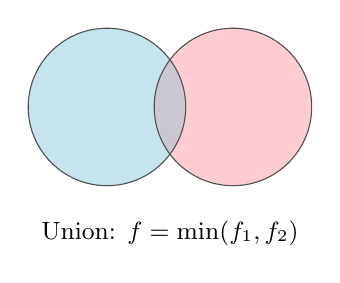
\begin{tikzpicture}[scale=1.0, every node/.style={font=\small}]
        \definecolor{shapeA}{RGB}{173,216,230}
        \definecolor{shapeB}{RGB}{255,182,193}
        \definecolor{overlap}{RGB}{200,200,210}
        \definecolor{outline}{RGB}{80,80,80}
        \fill[shapeA, opacity=0.7] (-0.8,0) circle (1);
        \fill[shapeB, opacity=0.7] (0.8,0) circle (1);
        \begin{scope}
          \clip (-0.8,0) circle (1);
          \fill[overlap, opacity=0.9] (0.8,0) circle (1);
        \end{scope}
        \draw[outline, thin] (-0.8,0) circle (1);
        \draw[outline, thin] (0.8,0) circle (1);
        \node at (0,-1.6) {Union: $f=\min(f_1,f_2)$};
      \end{tikzpicture}
    }

    % --- Intersection ---
    \only<2>{
      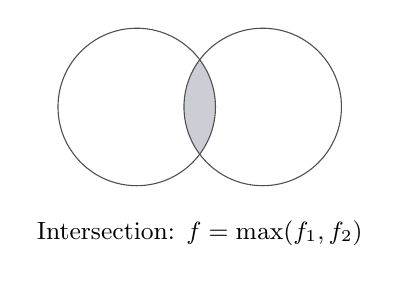
\begin{tikzpicture}[scale=1.0, every node/.style={font=\small}]
        \definecolor{shapeA}{RGB}{173,216,230}
        \definecolor{shapeB}{RGB}{255,182,193}
        \definecolor{overlap}{RGB}{200,200,210}
        \definecolor{outline}{RGB}{80,80,80}
        \begin{scope}
          \clip (-0.8,0) circle (1);
          \fill[overlap, opacity=0.9] (0.8,0) circle (1);
        \end{scope}
        \draw[outline, thin] (-0.8,0) circle (1);
        \draw[outline, thin] (0.8,0) circle (1);
        \node at (0,-1.6) {Intersection: $f=\max(f_1,f_2)$};
      \end{tikzpicture}
    }

    % --- Difference ---
    \only<3>{
      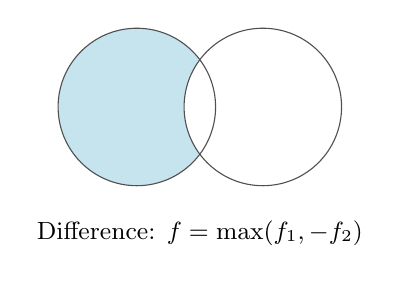
\begin{tikzpicture}[scale=1.0, every node/.style={font=\small}]
        \definecolor{shapeA}{RGB}{173,216,230}
        \definecolor{shapeB}{RGB}{255,182,193}
        \definecolor{outline}{RGB}{80,80,80}
        \fill[shapeA, opacity=0.7] (-0.8,0) circle (1);
        \begin{scope}
          \clip (-0.8,0) circle (1);
          \fill[white] (0.8,0) circle (1);
        \end{scope}
        \draw[outline, thin] (-0.8,0) circle (1);
        \draw[outline, thin] (0.8,0) circle (1);
        \node at (0,-1.6) {Difference: $f=\max(f_1,-f_2)$};
      \end{tikzpicture}
    }
  \end{column}

  % ===== Right Column: Explanations =====
  \begin{column}{0.4\textwidth}
    \only<1>{
      \begin{conceptbox}{Why min?}
        Inside if inside \textbf{either} shape.  
        Smaller signed distance (more negative) means  
        closer to the surface.
      \end{conceptbox}
    }

    \only<2>{
      \begin{conceptbox}{Why max?}
        Inside only if inside \textbf{both} shapes.  
        Larger distance ensures both must be negative.
      \end{conceptbox}
    }

    \only<3>{
      \begin{conceptbox}{Why max with $-f_2$?}
        Keep A’s interior, remove B’s interior.  
        Negating $f_2$ flips inside/outside for B.
      \end{conceptbox}
    }
  \end{column}
\end{columns}
